\section{Analyzing longitudinally collected isolates from patients of the University hospital Basel}
\subsection{Sample selection based on a pan genome analysis}
\begin{figure}
	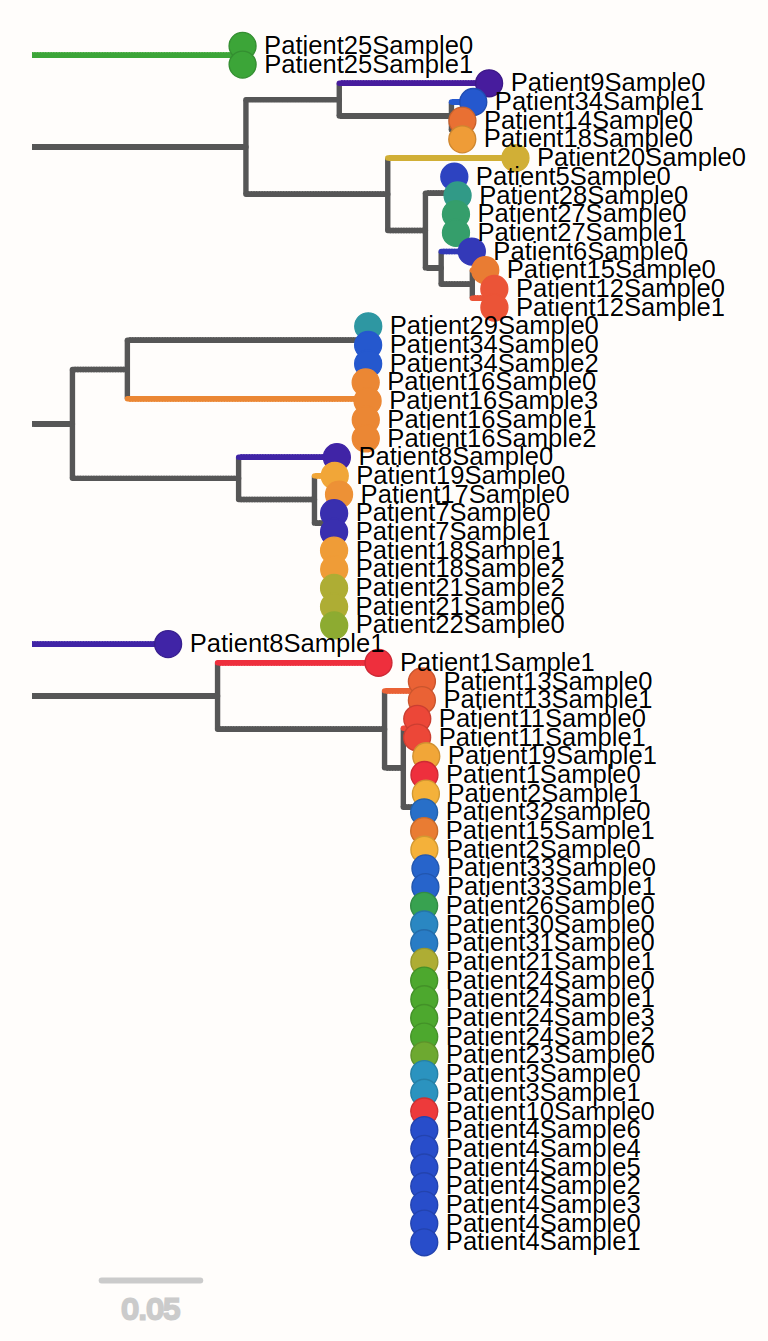
\includegraphics[scale=0.2]{181205_panXtree_overview.png}
	\caption{Phylogenic tree build with panX visualizing how cloesly related the pan genome of isolate is. }
	\label{figure:panX}
\end{figure}
The phylogenic tree in \ref{figure:panX} built with panX shows how cloesly related the pan genome of the different isolates is. 
Some isolates from the same patient (eg. Patient21, Patient8) have been isolated which map on different branches. This implements, that some patients got infected with a different strain over time. It's also visible, that some patients are affected by the same outbreak (different patients mapped on the same branch)
Since we want to identify changes in the genome caused by evolution of drug resistance, it's important that the patient was infected with the same strain over the entire sample period. Therefor only patients with all the isolated mapped on the same branch in \ref{figure:panX} could be included in the analysis.

What also had to be considered for selecting patients was that there was a significant change in the MIC over time for the isolates of the same patient. Usually MICs are determined by making a 1:1 dilution row, thus isolates where the MIC changed only by a factor of two, could not be included. 
Applying those criteria following samples were selected for the analysis:
\begin{table}
	\begin{tabular}{|c c c c c|}	
		\hline
		Accession & Sample date & MIC Cefepim & MIC Cefepim Sandra & Ceftazidim \\ [0.5ex]
		\hline\hline
		Patient12Sample0 & 9.9.14 & 4 & 16 & 0.75 \\
		Patient12Sample1 & 5.12.14 & 12 & 32 & 2 \\
		\hline
		Patient16Sample0 & 22.6.12 & 8 & 32 & 2\\
		Patient16Sample1 & 18.7.13 & 48 & 64 & 8\\
		Patient16Sample2 & 1.11.13 & 32 & 32 & 12\\
		\hline
		Patient24Sample0 & 02.05.11 & 4 & 16 & 1.5\\
		Patient24Sample1 & 08.15.11 & 16 & 32 & 1.5\\
		Patient24Sample2 & 11.28.11 & 3 & 8 & 1\\
		\hline
		Patient25Sample0 & 15.4.11 & 64 & None & 192\\
		Patient25Sample1 & 22.8.11 & 6 & 4 & 6\\
		\hline
		Patient33Sample0 & 26.9.14 & 24 & None & 16 \\
		Patient33Sample1 & 29.1.15 & 1 & 2 & 1.5\\
		\hline
	\end{tabular}
	\caption{Those patients have been selected because they differ significantly in MIC and are mapped on the same branch in panX}
	\label{table:samples_overview}	
\end{table}


